\chapter{Future Work}

SweetPea is a work-in-progress. The ultimate vision for SweetPea is to be a convinient system for describing many diverse types of experimental designs, and then quickly and seamlessly integrating the resulting experimental sequences with the users' existing experiment running pipelines. Ideally, SweetPea could be a tool in dialog with the user; the user should be able to use SweetPea to iterative explore the space of possible satisfiable experimental designs. To achieve this vision, SweetPea will need more high-level language features, and more runtime support for debugging unsatisfiable experiments.

One possible future direction for SweetPea which is orthogonal to this vision is to expand SweetPea to support experiments in other domains beyond psychology. Possible candidates for fields that could benefit from an experimental design description language are biology and machine learning; in both biology and machine learning, however, the experimental designs describe the set of trials to consider and lack a notion of ordering. This means that SweetPea would likely need to support more semantics for describing subsets of the crossing space, and applying constraints to these subsets.

%%% ~~~~~~~~~~~~~~~~~~~~~~~~~~~~~~~~~~~~~~~~~~~~~~~~~~~~~~~~~~~~~~~~~~~~~~~~~~~
\section{Future Language}


\paragraph*{Weighted Crossings}
It would be useful to have a mechanism to specify a way to over or under sample a full crossing. A usecase for this is a version of the Stroop experiment with 3 colors; in a full crossing there are 3 congruent stimuli, and 6 incongruent stimuli (see \figref{weighted_crossing}). It is well-motivated to want to balance the number of congruent and incongruent stimuli. One can imagine either undersampling the incongruent stimuli (choosing 3 of the 6 with uniform likelihood), or oversampling the congruent stimuli (such that each congruent stimuli occurs twice). More generally, it will be worth spending time in the future investigating more ways of specifying parts of the space of the full crossing.

\begin{figure}[t]
    \centerline{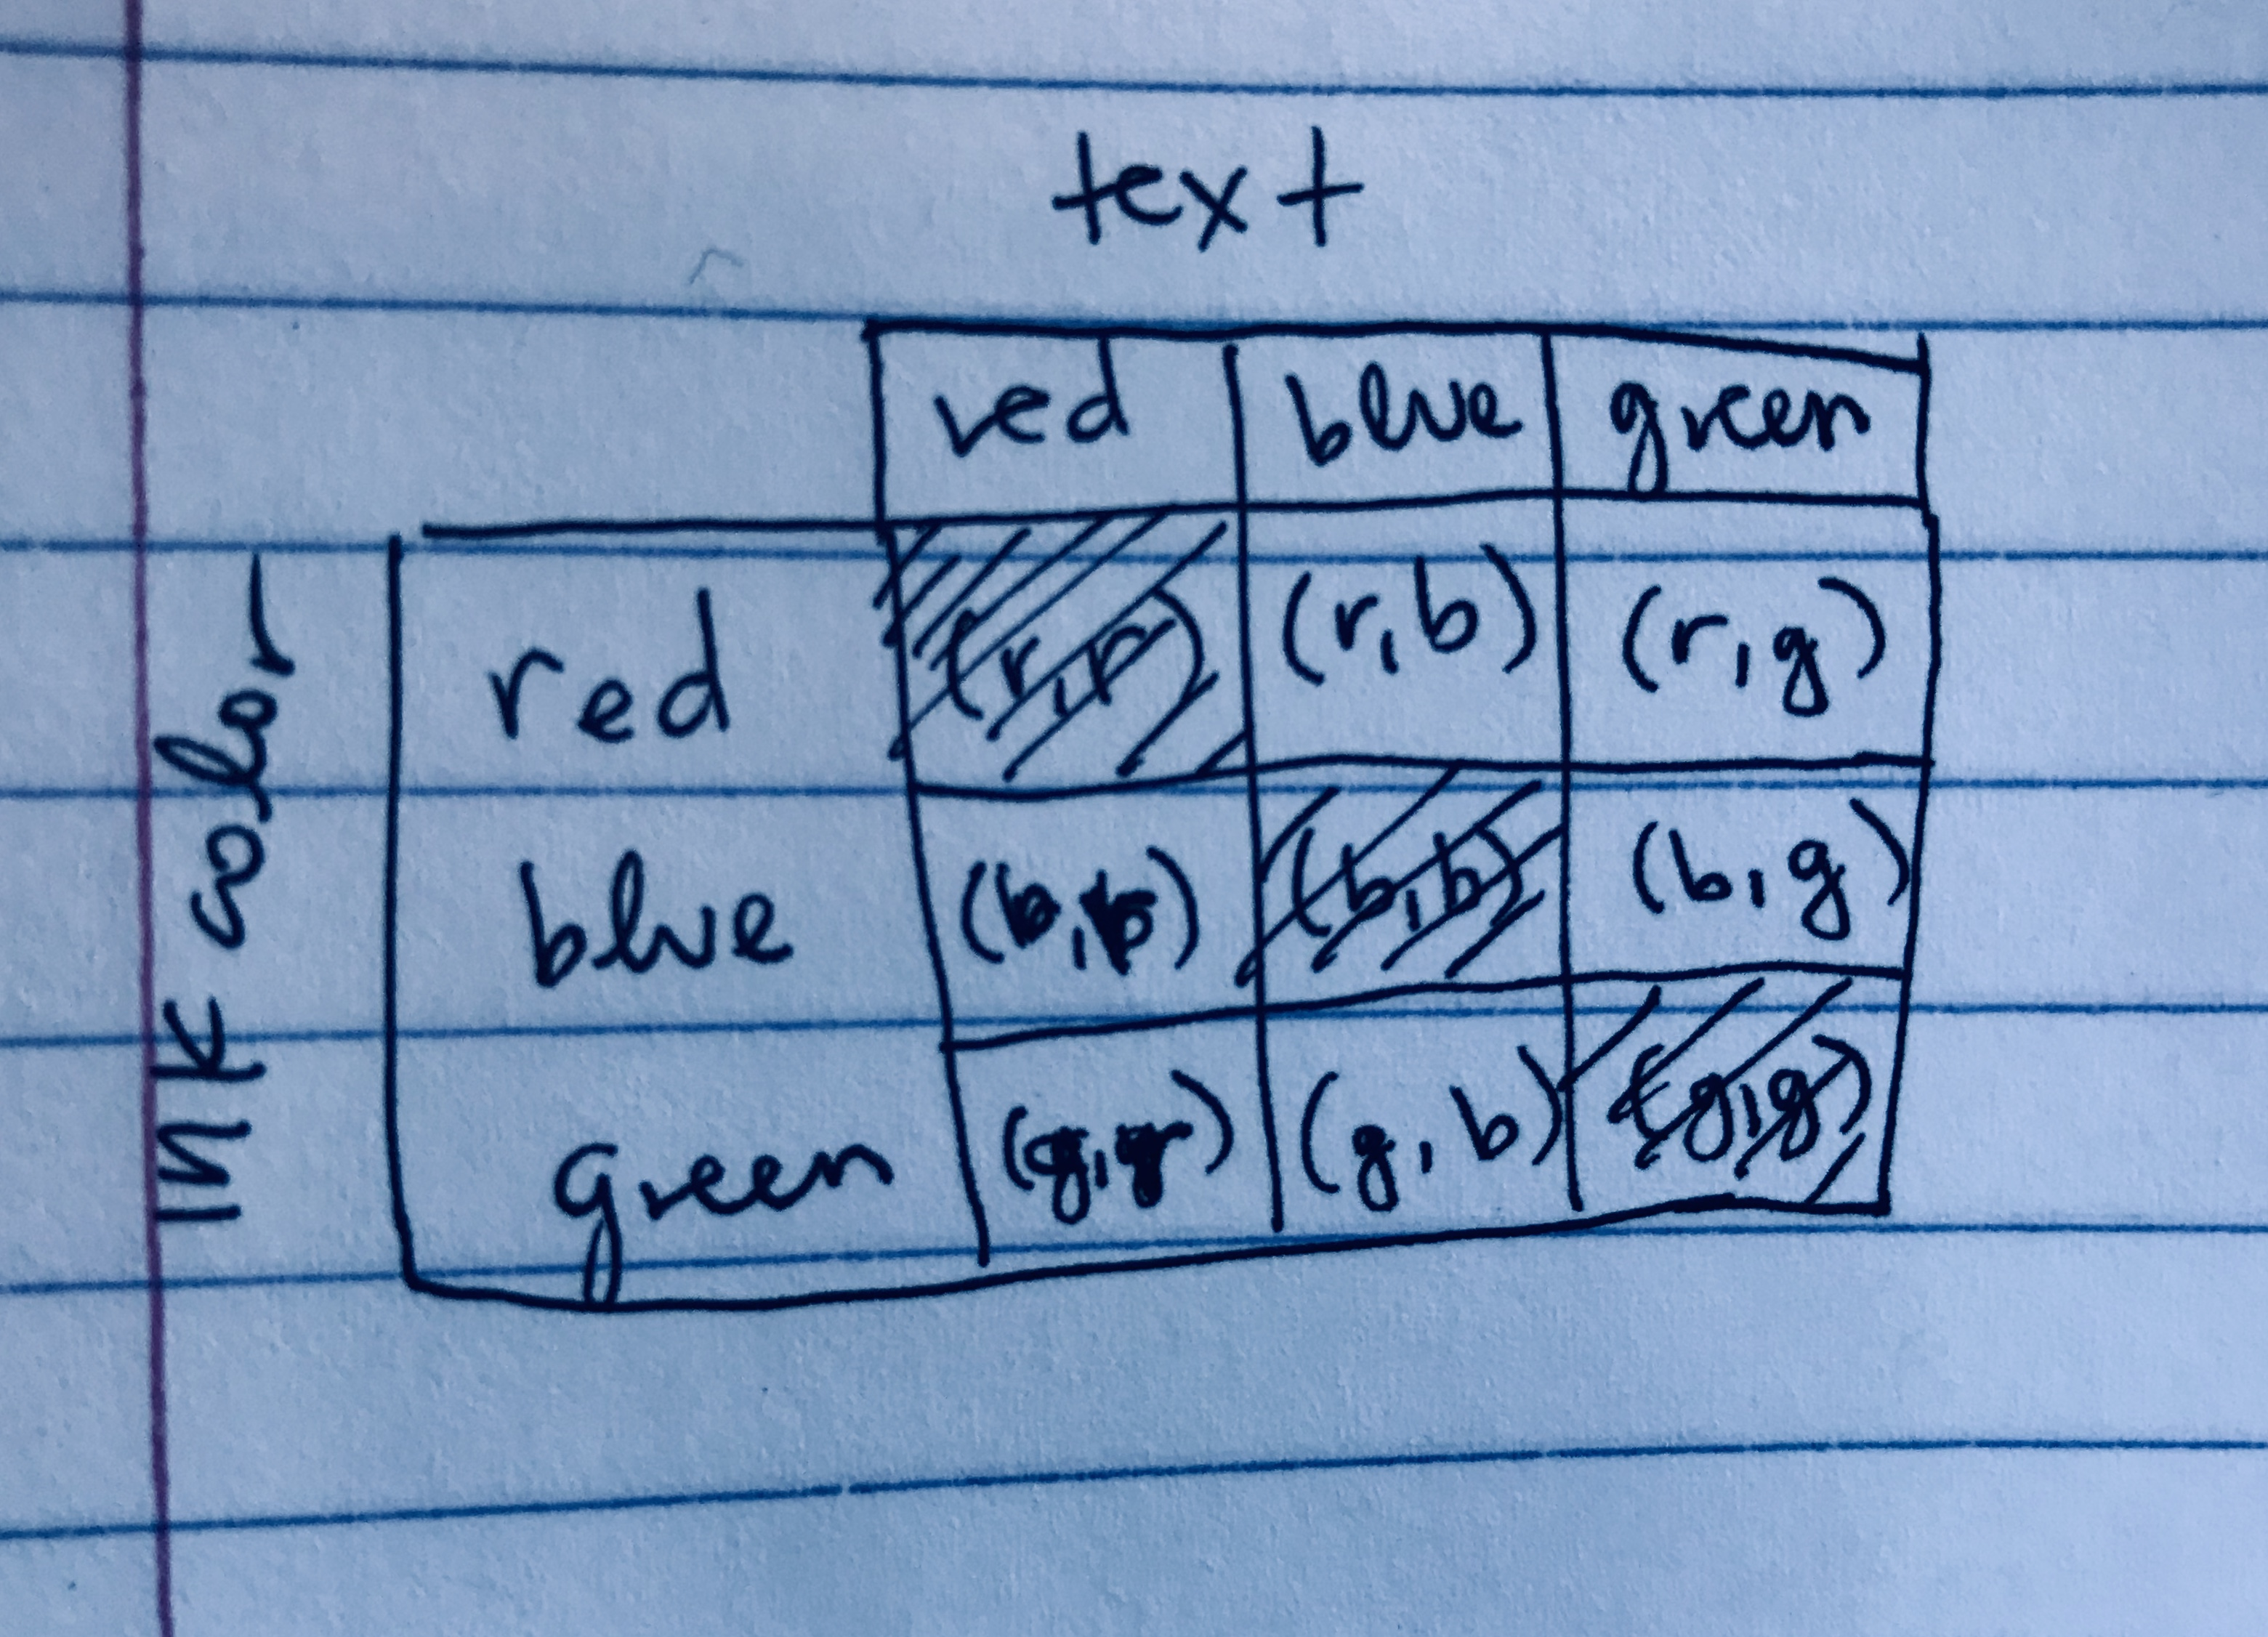
\includegraphics[origin=c,width=10cm]{fig_weighted_crossing}}
    \caption{Full crossing of a 3 color Stroop experiment. There are more congruent stimuli (along the diagonal) than incongruent stimuli.}%
    \label{fig:weighted_crossing}%
\end{figure}

\paragraph*{Sampling Continuous Factors}
Some experiments may contain levels which represent continuous values, such as TODO ASK SEBASTIAN. We can currently represent these experiments by binning the continuous values into a number of discrete levels-- but can we do better? This is challenging because the translation to SAT is necessarily discrete. Perhaps this could be supported as a pre- and post- processing step. The user could specify the continuous value, and SweetPea could performing binning, find a solution, and add random noise to the solution to simulate sampling from a continuous distribution.

\paragraph*{Automated Experimental Design}
In the spirit of declarative programming, it would be excellent to extend SweetPea to automatically derive the minimal set of counterbalancing conditions that satisfy the specified statistical analysis. Specifically, we may wish to provide an interface for the ANOVA (ANalysis Of VAriance) technique, which would allow researchers to state "contrast red with blue" instead of explicitly stating a design that does so. This higher-level interface will make it easier to specify experiments that accurately match the desired statistical analysis. Perhaps such an interface would also support iterative and interactive experiment specification. For instance, if multiple experiments match a desired statistcally analysis, perhaps the user can use SweetPea to explore the options and tradeoffs of each of those possible experiments.

%\paragraph*{Syntactic Sugar}
%- don't have to write the name of the factor when the level name is unique


%%% ~~~~~~~~~~~~~~~~~~~~~~~~~~~~~~~~~~~~~~~~~~~~~~~~~~~~~~~~~~~~~~~~~~~~~~~~~~~
\section{Future Runtime}


\paragraph*{Verified Core}

- the motivation for SweetPea is that it will make it easy to write correct experiments; that only holds if sweetpea doesn't itself have bugs.

- the tsietin transform is ripe for bugs because it's doing a non-human-readable transformation

- would be cool to formally verify that the transformations are correct


\paragraph*{Debugging unSAT experiments}

- why is this a problem: usability: if it's unSAT it just say unSAT but not why. Not very useful.

- can get "minimally unsat core" from SAT solver, maybe can translate that back to user-defined levels to guess what the problem is

\paragraph*{Iterative experimental design and Partial Satisfiability}

- really want to know if experiment is over-constrained

- maybe could try specify subsets to try to iterately find the most constraints that can be simultaneously satisfied -- solvers let you push / pop clauses

\paragraph*{Optimizations}

- xor constraints

- truth table simplification (Quine–McCluskey)

- choice of SAT encodings and variable v. clauses
